\chapter{Technológie}
\label{kap:technologie}

Kapitola pojednáva o voľbe vhodných technológii pre implementáciu jednotlivých cieľov práce. Detailom implementácie s použitím tu opísaných technológií je venovaná nasledujúca kapitola \ref{kap:implementacia}.

%%%%%
% %%% Editor kódu
%%%%%
\section{Editor kódu}
\label{kap:GrafickyProgramovaciJayzk}
Nakoľko je možnosť tvorby riadiaceho programu robota v grafickom programovacom jazyku (GPJ) našim ústredným cieľom, podriaďujeme mu výber ostatných technológií.

Koncept GPJ nie je novinkou. Začiatky rozvoja v tejto oblasti možno badať už v šesťdesiatych rokoch minulého storočia s nástupom počítačovej grafiky samotnej \cite{boshernitsan2004visual}. Myšlienka je to pritom takmer prirodzená, obrazové vnímanie je človeku blízke, vizuálne vnemy si ľahšie pamätáme, sú intuitívne. Ako označenie napovedá, tento typ jazyka sa vyznačuje práve tým, že nie je tvorený textovými prvkami, ako mnohé bežné jazyky. Elementy, z ktorých možno tvoriť program sú grafické, ide teda zväčša o rôzne ikony, šípky, obrazce či diagramy, ktorých rozmiestením a prepojením tvoríme kód.

Dnes je táto oblasť rozvinutá a grafické jazyky vieme klasifikovať do niekoľkých kategórií. Zaujímavou je kategória takzvaných \uv{čistých} grafických jazykov, ktoré sú kompilované z grafickej formy priamo do strojového kódu. Pre našu aplikáciu je však podstatná druhá z hlavných kategórií, obsahujúca \uv{hybridné textovo--vizuálne systémy}, do ktorej spadajú i tie, umožňujúce tvorbu programu vo vizuálnej podobe, ktorá je ale následne preložená do textovej reprezentácie v niektorom z textových jazykov. Práve tento koncept je pre našu aplikáciu vhodný, vytvoríme GPJ s adekvátnymi prvkami, preložiteľnými to jazyka C, ktorému \uv{rozumejú} riadiace jednotky robotov.

Potenciál GPJ je predovšetkým v možnosti interaktívnej tvorby kódu (napríklad formou drag and drop), ich názornosti a jednoduchosti, umožňujúcej v prípade potreby vysokú abstrakciu od textovo orientovaného jazyka, do ktorého sú prekladané. V mnohých prípadoch sú tak ideálnym riešením pre začínajúcich programátorov aj ako istý medzistupeň pri výučbe programovania v textovom jazyku. V porovnaní s textovou formu sú grafické jazyky v nevýhode hlavne v komplexite, obrazová reprezentácia viac zaťažuje pamäť i procesor. S narastajúcou dĺžkou kódu môžu byť tiež menej prehľadné, ťažko udržiavateľné i rozšíriteľné.

% LabVIEW
\subsubsection{LabVIEW}
Laboratory Virtual Instrument Engineering Workbench (LabVIEW) je výtvorom spoločnosti National Instruments, zaoberajúcou sa tvorbou softvéru a zariadení pre automatické testovanie. Produkt má širšie spektrum použitia, mimo iného je s jeho pomocou možno vytvárať riadiace programy pre vnorené systémy v jazyku G \cite{LabVIEW}.

Základným prvkom jazyka je takzvaný VI --- \uv{virtuálny prístroj} (angl. Virtual Instrument). VI môže predstavovať celý program alebo byť súčasťou väčšieho programu. Pre každý VI používateľ definuje prvky \uv{predného panela}, zobrazujúceho stav prístroja. Pomocou panela je tiež možné definovať vstupy a po výpočte získať výstupné hodnoty. VI ďalej tvorí \uv{diagram blokov}, definujúci správanie VI vo vizuálnej podobe. Bloky reprezentujú funkcie, k dispozícii sú rôzne, od jednoduchých aritmetických operácií až po komplexnejšie. V diagrame je umožnený prístup k vstupom definovaným prostredníctvom predného panela. Bloky sú prepájané \uv{vodičmi}, reprezentovanými čiarami, znázorňujúcimi tok dát. Postup vyhodnocovania vstupu je založený na dostupnosti dát --- blok sa vyhodnotí v momente, keď sú preň dostupné všetky vstupné hodnoty a výsledok je následne dostupný pre ďalšie prepojené bloky alebo odoslaný na výstup (predný panel).

Na LabVIEW je založená aplikácia firmy Lego na tvorbu riadiacich programov robota Mindstorm (kapitola \ref{sub:LegoMindstorms}). Nevýhodou pre našu aplikáciu je najmä spoplatnenie tohto softvéru, napriek tomu je to jedno z možných riešení.

% Blockly
\subsubsection{Blockly}
Blockly je produktom firmy Google. Ide o knižnicu vytvorenú v jazyku JavaScript ako nástroj na tvorbu GPJ. Dostupná je v duchu open--source bez poplatkov a nesie licenciu Apache 2.0, ktorá ju umožňuje použiť k akémukoľvek účelu aj v modifikovanej verzii. Jazyky tvorené touto knižnicou spadajú do kategórie hybridných GPJ, kód v nich tvorený je prekladaný do textového jazyka a až následne kompilovaný do strojového kódu.

\begin{figure}
\centerline{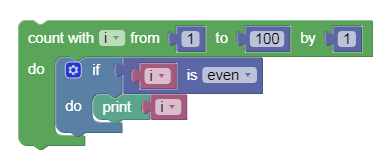
\includegraphics[width=0.7\textwidth]{images/blocky-example}}
\caption[Použitie blokov v knižnici Blockly]{Použitie blokov v knižnici Blockly}
\label{obr:blockly-example}
\end{figure}

Základným stavebným prvkom jazykov vytvorených pomocou Blockly je \uv{blok}, ktorý možno prirovnať k dieliku puzzle alebo akejsi kachličke \cite{pasternak2017tips}. Bloky sú rôznych typov a zvyčajne reprezentujú prvky cieľového textového jazyka ako cykly, premenné, procedúry, aritmetické operácie a iné. Dôležitou súčasťou novovzniknutých jazykov sú ale bloky vytvorené špecificky pre danú oblasť. V našom prípade to môžu byť dieliky sprístupňujúce používateľov rôzne funkcie robota ako ovládanie motorov či vydávanie zvukových signálov. Výsledný kód je tvorený spájaním blokov do väčších celkov. Príklad bloku vykonávajúceho (neefektívny) výpis párnych prirodzených čísel menších alebo rovných ako sto môžete vidieť na obrázku \ref{obr:blockly-example}.

Blockly pozostáva z dvoch hlavných častí, definícií blokov a definícií generátorov, zabezpečujúcich preklad do cieľového textového jazyka. Od vývojárov sú k v knižnici k dispozícii \uv{od výroby} bloky a generátory pre jazyky JavaScript, Lua, PHP, Dart, a Python. I keď našim cieľom je jazyk C, existujúce časti nám môžu byť nápomocné.

Výhodou je vysoká prispôsobiteľnosť blokov po dizajnovej stránke, ale tiež možnosť konfigurácie spojov medzi dielikmi tak, aby vynucovali syntaktické pravidlá cieľového jazyka a vykonávali typové kontroly. Benefitom je tiež neutíchajúci aktívny vývoj a dostupnosť dokumentácie. Integrovanie knižnice do aplikácie tiež netvorí prekážku, nakoľko JavaScript možno spúšťať v prehliadačoch, ktoré sú bežnou súčasťou vývojových platforiem ako komponent \uv{WebView}. Knižnica je nasedená v mnohých kontextoch, osvedčená je v oblasti výučby (napríklad projektom Scratch) ale i robotiky, tu je dôkazom napríklad aplikácia RoboBlockly alebo už spomínaný projekt Otto Blockly (kapitola \ref{sub:OttoBlockly}) a aj preto sme sa rozhodli pre jej použitie v našej práci.


%%%%%
% %%% Aplikácia
%%%%%
\section{Implementačný jazyk aplikácie}
Výber knižnice Blockly ako nástroja pre tvorbu grafického jazyka nabáda k vývoju internetovej aplikácie a nie desktopovej. Napriek tomu, že ide o JavaScript knižnicu, podriaďujeme ju desktopovej aplikácií, nakoľko bežný internetový prehliadač nedisponuje funkciami potrebnými pre splnenie ďalších cieľov našej práce. Problematickou je napríklad komunikácia s robotom prostredníctvom sériového portu, ku ktorému nezvykne byť v prehliadačoch možný prístup pre bezpečnostné riziko. 

Rovnako môže byť komplikované spúšťať iné desktopové aplikácie (napríklad prístupom k príkazovému riadku), čo je nevyhnutné pre spustenie Arduino kompilátora po vytvorení riadiaceho programu. Implementácia týchto funkcionalít v rámci internetovej aplikácie nie je nemožná, no vyžadovala by napríklad vývoj a inštaláciu rozšírení webových prehliadačov.

Zohľadňujúc požadované funkcionality, popularitu jazykov a skúseností autorov práce, je voľbou pre implementáciu jazyk Java. Java poskytuje rozsiahly systém na tvorbu grafických používateľských rozhraní --- JavaFX. Ten umožňuje oddeliť v kóde definície logiky a vzhľadu (rozloženia), na ktoré slúži formát XML. Vzhľad a správanie jednotlivých grafických prvkov je pritom možné ľahko ovládať i v Java kóde. Súčasťou systému JavaFX je komponent webview, slúžiaci ako prehliadač, v ktorom možno spustiť grafické rozhranie knižnice Blockly a tiež dovoľuje obojsmernú komunikáciu medzi jazykom JavaScript a Java.

Java tiež umožňuje ľahko spúšťať externé programy a komunikovať s nimi prostredníctvom ich CLI. Nechýbajú v nej ani mechanizmy na komunikáciu cez sériový port.


%%%%%
% %%% Vizualizácia
%%%%%
\section{Vizualizácia}
Spúšťanie vytvorených programov v jednoduchej simulácii je jednou zo zamýšľaných funkcionalít našej aplikácie. Priamočiarym postupom implementácie je použitie API ako Vulkan alebo OpenGL pre komunikáciu s GPU a návrh grafických prvkov od základu. Takto by však bolo nutné vytvoriť pomerne rozsiahly modul na nízkej úrovni, čo nie je pre našu jednoduchú simuláciu nutné. Existuje hneď niekoľko riešení vyššej úrovne, ponúka sa použitie rôznych knižníc, simulátorov či herných programov.

% Simulátor
\subsection{Simulátor}
Prirodzeným prístupom k riešeniu modulu simulácie je použitie existujúceho robotického simulátora. K dispozícii je ich hneď niekoľko, keďže sa bežne používajú ako pomôcka na testovacie účely pred skonštruovaním zariadení.

\textit{Webots} je jedným z dostupných simulátorov. Ide o open--source desktopovú aplikáciu umožňujúcu navyše i modelovanie a programovanie prístrojov \cite{Webots}. Program robota môže byť vytvorený v rôznych jazykoch (C, C++, Python , Java, MATLAB, ROS), prostredie simulácie možno upravovať v jazyku VRML97 (Virtual Reality Modeling Language). Súčasťou je podpora senzorov a simulácia fyzikálnych javov.

Ďalšími známymi simulátormi sú Gazebo, Visual Components, RoboDK, V-REP, RobotStudio, WorkcellSimulator či RoboLogix. Jedná sa však o programovacie nástroje, zväčša komplexné a hlavne samostatné aplikácie s vlastným GUI. Umožňujú detailnú simuláciu a pre účely jednoduchej vizualizácie nie sú vhodné. Od ich použitia nás odrádza nie len zbytočne vysoká komplexita ale i komplikácie spojené s integráciou do našej aplikácie.

% Game engine
\subsection{Herný program}
\label{sub:herny-program}
Herné programy (angl. game engines) poskytujú iný prístup k riešeniu modulu simulácie. Zvyčajne sú v nich k dispozícii všetky potrebné funkcionality bežne prítomné v už spomínaných simulátoroch (niektoré simulátory sú dokonca založené na hernom programe). Rovnako poskytujú nástroje pre konštrukciu a vykreslenie trojrozmerného virtuálneho prostredia, do ktorého možno pridávať ďalšie objekty. V celom prostredí možno uplatňovať a simulovať fyzikálne zákony a javy ako gravitácia, trenie či zrýchlenie. \uv{Herný} charakter týchto produktov je zvyčajne viditeľný najmä v poskytovaných funkcionalitách ako podpora sieťovej komunikácie či rozoznávanie gest v GUI.

Najväčšou výhodou je pomerne jednoduchá integrácia do aplikácie, keďže herné programy majú tiež formu softvérových rámcov a knižníc. Po stanovení implementačného jazyka je vhodné nájsť \uv{hernú knižnicu} vytvorenú v rovnakom jazyku. Inšpiráciou sú nám odporúčania uvedené na stránke LWJGL (Lightweight Java Game Library), knižnice, ktorá umožňuje v Java aplikáciách prístup k spomínaným API ako OpenGL či Vulkan \cite{LWJGL}. Tu autori pre začínajúcich vývojárov v oblasti sami odporúčajú použitie herných programov založených na tejto knižnici. Spomínané sú dva --- LibGDX a jMonkeyEngine.

\subsubsection{LibGDX}
LibGDX je softvérovým rámcom (angl. framework), umožňujúcim vývoj hier pre viacero platforiem súčasne. Založený je na OpenGL, kód je zverejnený v duchu open-source a licencia Apache 2.0 nás od jeho použitia rovnako neodrádza. Pre používateľov --- začiatočníkov je k dispozícii rozsiahla dokumentácia (Javadoc) a rôzne návody. Zaujímavosťou je aplikácia na vytvorenie základnej kostry výslednej \uv{hry} (u nás simulácie), ktorá po zadaní niekoľkých parametrov výrazne uľahčí úvodné nastavenie a možno tak rýchlo prejsť k vývoju hry samotnej (ako herná logika či rozmiestnenie objektov) \cite{LibGDXProjectGenerator}.

\subsubsection{jMonkeyEngine}
\label{subsub:jMonekyEngine}
jMonkeyEngine (ďalej ako \uv{jME}) je možné k projektu ľahko pridať vo forme knižníc pomocou nástroja Maven. Podobne ako LibGDX nás v jeho použití neobmedzuje ani licencia (pripojená BSD 3--Clause licencia umožňuje použitie produktu s modifikáciou i na komerčné účely) ani poskytnuté funkcionality. Nechýba dokumentácia, návody pre začiatočníkov, vlastný SDK a IDE.

Oba herné programy pokrývajú naše požiadavky a na internetových fórach je ich možné veľakrát nájsť ako ekvivalenty, pre ktoré sa pri vývoji hry ťažko rozhodnúť. Častým odporúčaním však je voľba jME, ak má byť výsledný produkt zameraný prevažne na trojrozmernú grafiku, čo platí aj v našom prípade.

K výberu jME, ako technológie pre implementáciu simulácie, prispel i článok priamo opisujúci simulátor robotov vytvorený pomocou jME --- jmeSim \cite{jmeSim}. I keď je údajne tento simulátor open--source, nedopátrali sme sa k jeho zdrojovému kódu. Napriek tomu považujeme článok za dôkaz, že má zmysel snažiť sa o simuláciu v hernom programe, a jME je pre tento účel použiteľnou technológiou.

Integrovať simuláciu do našej aplikácie pomôžu existujúce riešenia ako JME3-JFX \cite{jmejfx}, ktoré umožňujú vykresľovanie grafického obsahu simulácie v jME priamo do komponentu JavaFX scény.

\subsubsection{Princíp a možnosti jMonkeyEngine}
Ústredným určením jME je v podstate sprostredkovanie nízkoúrovňového prístupu k funkciám grafickej karty na úrovni vyššej. Programátorovi navyše poskytuje niekoľko užitočných abstrakcií a dátových štruktúr \cite{jmeDocumentation}. Základom hry (simulácie) je \textit{scéna}, trojrozmerné prostredie, v ktorom sú umiestňované \textit{uzly} usporiadané v stromovej štruktúre. Prázdnu scénu tvorí jediný uzol --- \textit{root}, ku ktorému sú pri výstavbe scény priraďované ďalšie. Uzol je abstraktným, neviditeľným bodom v priestore, má svoju polohu, rotáciu a mierku (angl. scale). Umožňuje logické rozmiestnenie viditeľných prvkov zlučovaním do skupín (viacero uzlov môže mať spoločného rodiča) a tým i hromadnú manipuláciu s mu podriadenými uzlami. Poloha je určená súradnicovým systémom (obrázok \ref{obr:coordinate-system}).

\begin{figure}
\centerline{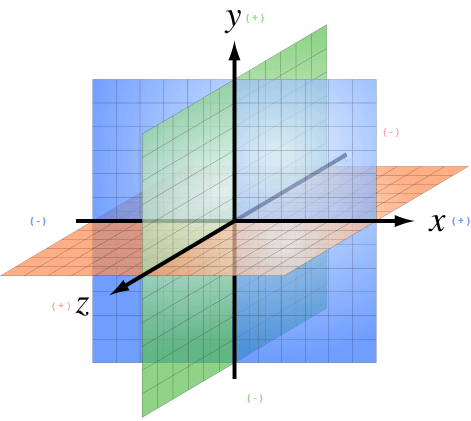
\includegraphics[width=0.4\textwidth]{images/coordinate-system}}
\caption[Súradnicový systém scény v jMonkeyEngine]{Súradnicový systém scény v jMonkeyEngine}
\label{obr:coordinate-system}
\end{figure}

Viditeľnými časťami scény sú \textit{geometrie}. Súčasťou scény sa stávajú priradením do už spomínaného stromu uzlov, a podobne ako uzlom je im možno určiť transláciu, rotáciu a mierku. Viditeľnú časť geometrie tvorí 3D tvar a materiál. Tvar môže byť jednoduchým modelom geometrického telesa (kocky, gule alebo iného) alebo komplexným modelom --- \textit{sieťou} (angl. mesh) tvorenou drobnými polygónmi (zvyčajne trojuholníkmi) aproximujúcimi komplikovanejší tvar povrchu zobrazovaného objektu. Materiál určuje vlastnosti povrchu modelu ako svetlosť, priehľadnosť či lesklosť, a pomocou neho môže byť na model aplikovaná textúra. S materiálmi úzko súvisí svetlo. V scéne možno definovať zdroje svetla (umiestnenie, prípadne smer žiarenia), podľa ktorých pôsobenia sú následne zobrazované viditeľné prvky scény.

Dôležitou súčasťou scény je \textit{kamera}. Tá určuje, čo sa zobrazí na výstupe, v priestore má definovanú polohu, orientáciu, a dohľad. Výhodou definície dohľadu sú hlavne úspory výpočtových zdrojov, nakoľko pre prvky mimo záber nie je nutné počítať detaily zobrazenia.

Pre manipuláciu s uzlami a geometriami sú v jME k dispozícií rôzne dátové štruktúry. Používajú sa najmä vektor a kvaternión (angl. quaternion), pomocou ktorých možno meniť polohu a rotáciu objektov. K dispozícii sú tiež funkcie umožňujúce konštrukciu zložitejších štruktúr (kvaternión) z jednoduchších reprezentácií (matica alebo množina uhlov pri definícii rotácie). Dostupné sú i operácie nad týmto štruktúrami.

Kód simulácie sa skladá z dvoch hlavných častí, metód pre \textit{inicializáciu} a \textit{aktualizáciu}. Metóda inicializácie je volaná práve raz, pri spustení aplikácie. Jej určením je príprava scény, vykonávajú sa tu úkony ako počiatočné rozloženie uzlov, načítanie modelov, nastavenie osvetlenia. Metóda aktualizácie je zodpovedná za manipuláciu s prvkami scény počas behu aplikácie. Je cyklicky volaná obslužným vláknom aplikácie, s parametrom určujúcim čas od posledného volania (angl. time per frame --- TPF). Údaj je nápomocný napríklad pre zabezpečenie plynulého pohybu modelov v scéne, nakoľko jednotlivé volania metódy nemusia prebiehať v uniformných intervaloch. Po každom volaní metódy aktualizácie nasleduje vykresľovanie scény podľa aktuálneho rozloženia.

Simulácia fyzikálnych procesov je v jME možná pre spojenie s knižnicou Bullet, ktorá zodpovedá za monitorovanie stavu a prepočet polohy fyzikálnych objektov. V programe sú geometriám, ktoré majú byť súčasťou fyzikálnej simulácie vytvorené \textit{fyzikálne ovládače} a následne je riadenie ich pohybu podriadené výsledkom výpočtov fyzikálneho modulu. Fyzikálnym objektom môžu byť priradené doplňujúce parametre ako hmotnosť, trenie povrchu, aktuálne pôsobiaca sila, rýchlosť a podobne. Dôležitým konceptom pri simulácii fyzikálnych procesov (najmä v reálnom čase) je zjednodušovanie modelu simulovaného objektu. Nemusí pritom ísť o zjednodušenie viditeľnej časti, fyzikálny modul môže pre účely výpočtu používať iný, jednoduchší tvar telesa ako je zobrazovaný používateľovi, takzvaný \textit{kolízny tvar}. Bullet zohľadňuje zotrvačnosť telies a umožňuje definovať vzťah medzi dvoma uzlami pomocou neviditeľného \uv{kĺbu}, obmedzujúceho rotáciu v definovaných osiach a rozmedzí pri pôsobení síl na ním spojené uzly.

